\documentclass[12pt]{article}

% This first part of the file is called the PREAMBLE. It includes
% customizations and command definitions. The preamble is everything
% between \documentclass and \begin{document}.

\usepackage[margin=1in]{geometry}  % set the margins to 1in on all sides
\usepackage{graphicx}              % to include figures
\usepackage{subfig}
\usepackage{epstopdf}
\usepackage{amsmath}               % great math stuff
\usepackage{amsfonts}              % for blackboard bold, etc
\usepackage{amsthm}                % better theorem environments
\usepackage{hyperref}
\usepackage{changepage}




\begin{document}

\begin{center}
{\bf \Large Visual Saliency: Mid-point Check Report}  \\
\vspace{.1in}
{\em Sijie Ling, Shupei Zhang, Mehdi Akbarian Rastaghi}
\end{center}
%\setlength\parindent{0pt}
\section{Introduction}

Visual saliency is the extent of attraction of objects to our visual system. 
The human visual system can focus on the most salient stimuli and pay less attention to the rest. 
For example, a running dog in a still background will attract more of our attention. 
A reason for developing such a feature is that the amount of data we receive through our eyes exceeds our ability to process data. 
Although human brain capabilities evolved through time, it is a big challenge for our brain to process this tremendous amount of data efficiently. 
Hence, visual saliency can help us to identify the most imminent threat, danger, or events needing our attention in general. 
Technically, it reduces the load on our visual system. 

The study of visual saliency can help us to have a deeper understanding of the human visual system. 
Researching in this area can lead to many applications, such as image/video segmentation, image/video compression, foreground annotation, perceptual quality assessment, etc. \cite{congReviewVisualSaliency2019}.  
To shed more light, let's start with a case. 

Most of the current video coding methods are using block-based compression. 
As an example, spatial and temporal redundancy is reduced through intra-frame coding and inter-frame coding, respectively\cite{sullivanOverviewHighEfficiency2012}. 
While these methods play a vital role in the comparison area, video encoders can further increase the compression ratio by incorporating visual saliency models. 
This can be achieved by decreasing the quality of regions of low interest, like the background. 
Because it is hard for us to notice the changes in those regions, the perceptual visual quality will likely remain the same.

Another advancement of visual saliency is in the game industries. 
Visual saliency study might help game developers in optimizing the performance of their games. 
Due to the difference in attraction of different regions, not all areas need to be rendered in the highest quality, which leads to a better graphics performance. 
Therefore, considering all contribute of visual saliency techniques motivates us to do some research in this area. 

In this project, we will explore how to use attention mechanisms in computer vision, like \cite{zhangSelfAttentionGenerativeAdversarial2019a},
to help capture global dependencies, and thus improve the saliency prediction performance. 
The model will be an end-to-end model, where the input is a color image and the output is a saliency map.
The saliency map is the same size as the input image, with scores from 0 to 1 assigned to 
every pixel, indicating the extent of attraction of the corresponding pixel in the input image.
Higher values correspond to higher visual saliency levels.
One example of the original image and its corresponding saliency map is shown in Fig. \ref{img:data_example}.
\begin{figure}[!h]
    \centering
    \subfloat[][Original]{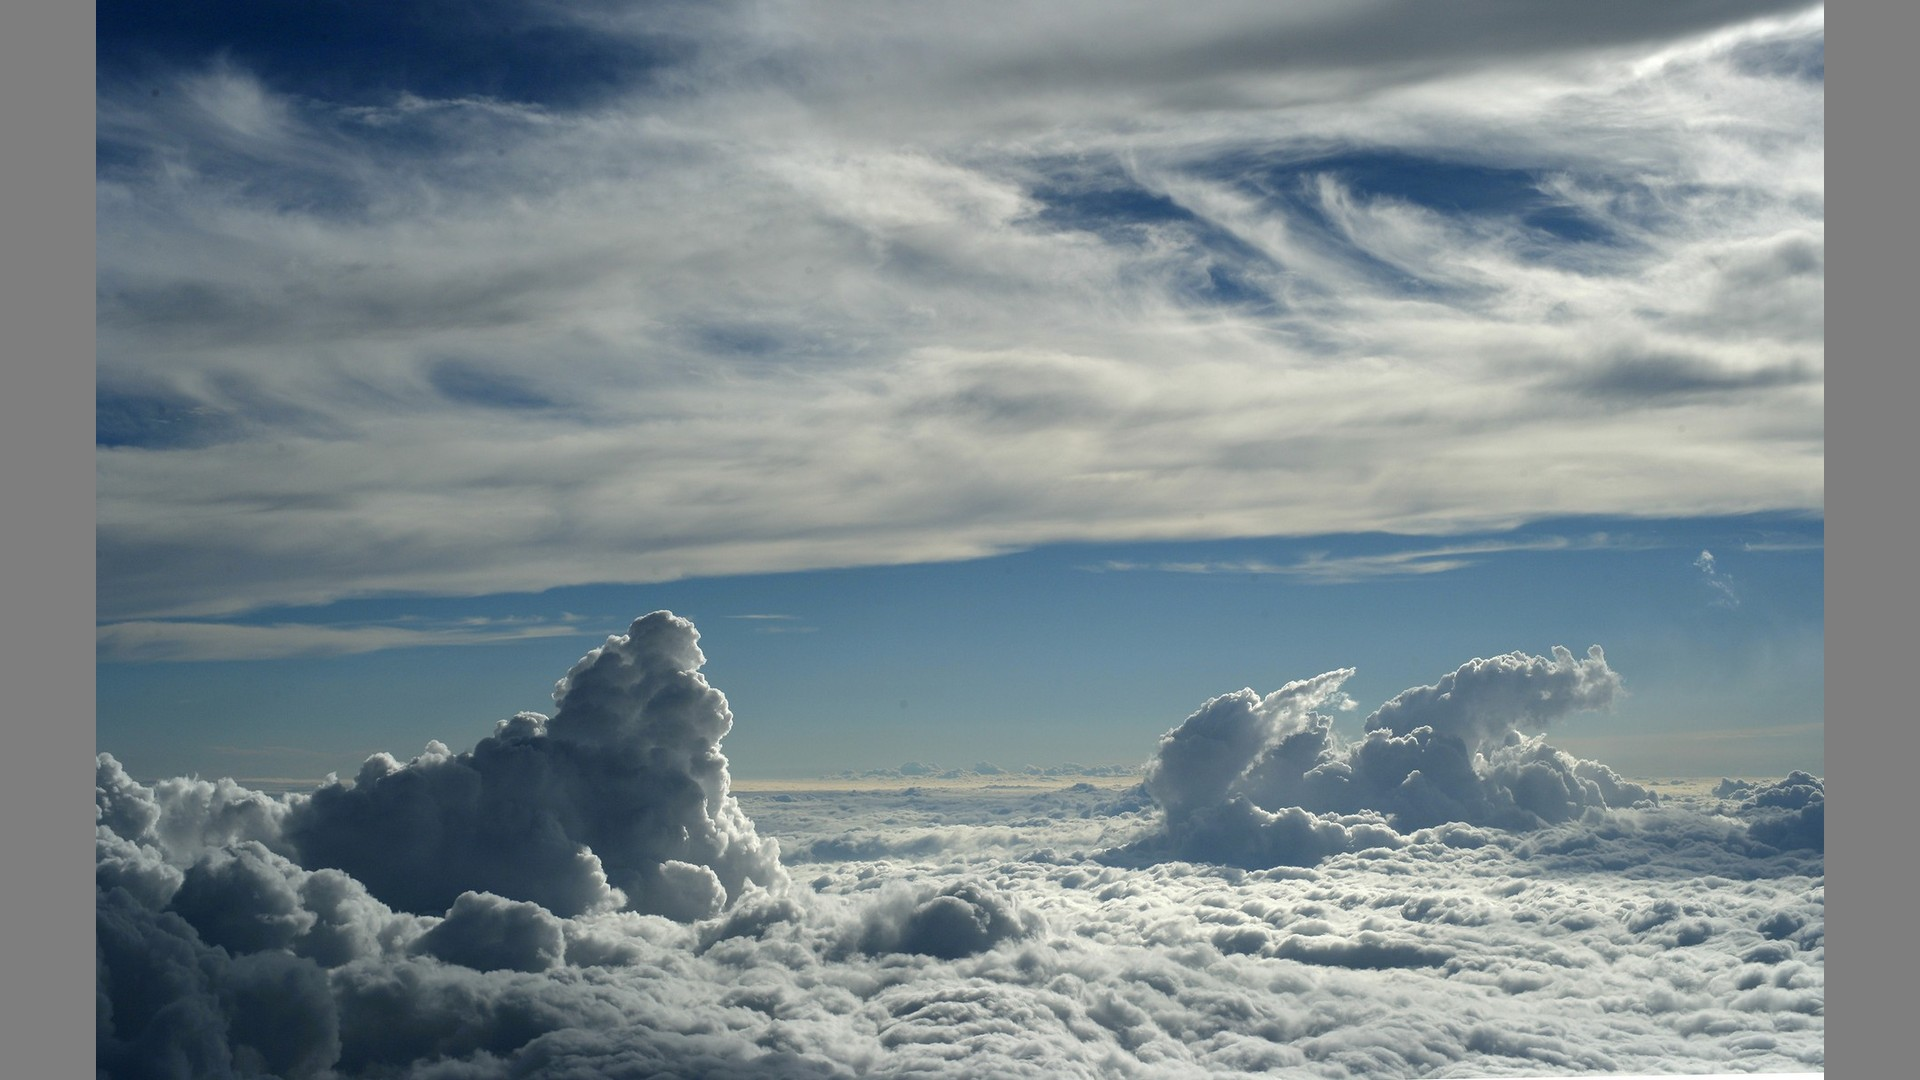
\includegraphics[width=3in]{imgs/example1_original.jpg}}
    \hspace{5mm}
    \subfloat[][Saliency map]{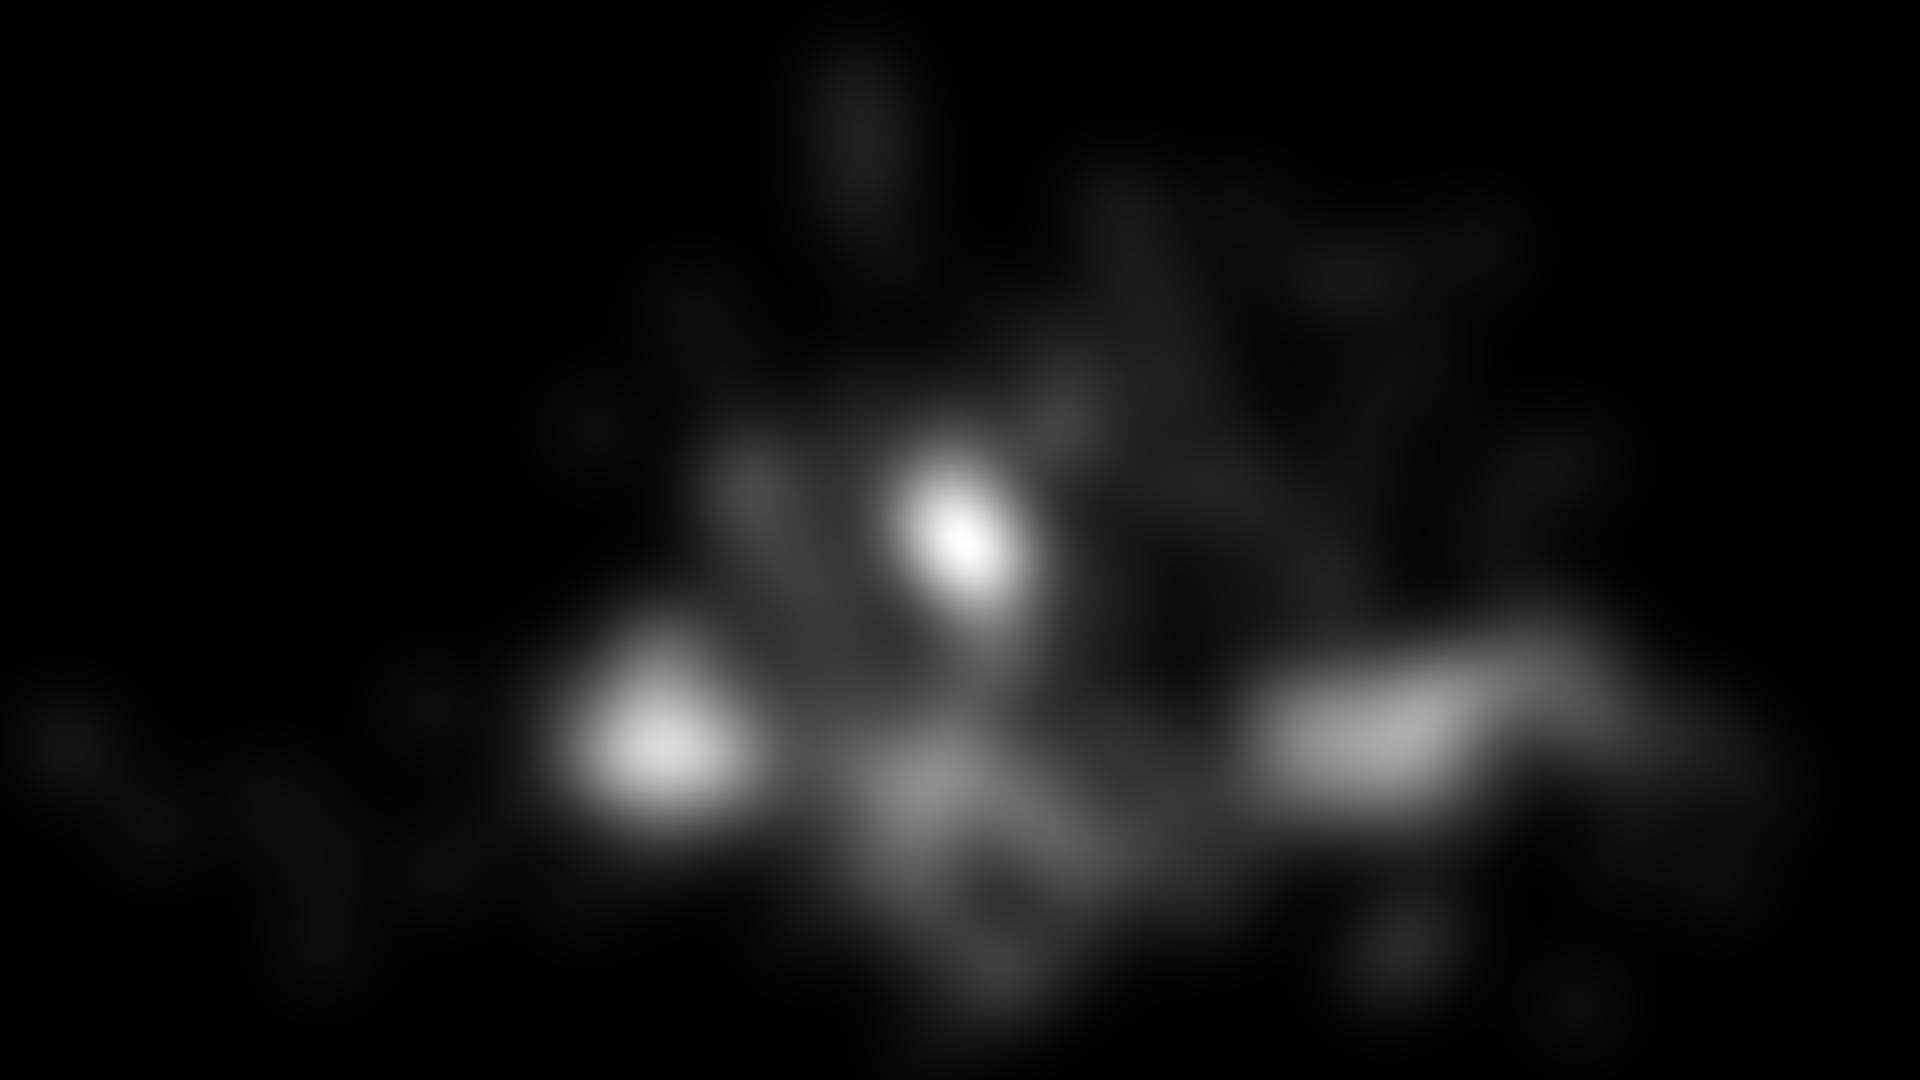
\includegraphics[width=3in]{imgs/example1_saliency.jpg}}
    \caption{Data example}
    \label{img:data_example}
\end{figure}


\section{Related Work}

Visual saliency detection methods can be categorized into two classes: bottom-up models and top-down models \cite{congReviewVisualSaliency2019}.
Before deep learning was widely applied in this field, most of the early methods are bottom-up models.
Those early methods usually involve biological and psychological research about visual attention mechanism. And those two approaches match the common beliefs about biological process of human vision.
In general, those models try to establish links between visual saliency and low-level image features, such as color, contrast, brightness etc. The Itti. model\cite{ittiModelSaliencybasedVisual1998}
is one of the earliest models of this kind, which predicts visual saliency from linear combination of features calculated from color, intensity and orientation.
Some other techniques are also used to achieve better results, such as frequency domain analysis, sparse representation, cellular automata etc. \cite{congReviewVisualSaliency2019}

Top-down models, in the other hand, try to find what factors have the most impact on visual saliency. Those models use visual saliency datasets, which contain images and their saliency annotations
, and analyze them in a data-driven fashion.
In recent years, deep learning is introduced into this area and has boosted the performance of saliency prediction a lot.
Vig et al. \cite{vigLargeScaleOptimizationHierarchical2014} proposed the first neural network for saliency prediction, combining convolutional neural network (CNN) and support vector machine (SVM). Later, researchers start to use transfer learning for saliency 
detection tasks. Very deep convolutional networks (VGG) is used in multiple models \cite{kruthiventiDeepFixFullyConvolutional2015, kummererDeepGazeIIReading2016, corniaPredictingHumanEye2018}, and some of them incorporate gaussian prior for performance improvement.
Generative adversarial networks also achieve good results in saliency prediction \cite{panSalGANVisualSaliency2018, cheHowGazeInfluenced2020}.

Transformer is a network based on attention mechanisms, and is first applied in natural language processing (NLP) for its ability to model long range and multi-level information \cite{bahdanauNeuralMachineTranslation2016a, vaswaniAttentionAllYou2017a}.
They are later introduced for computer vision tasks and show strong potential in modeling non-local dependencies in images \cite{zhangSelfAttentionGenerativeAdversarial2019a}.
But this technique has not been applied in visual saliency tasks so far.

Our trial of applying attention mechanism to CNNs to improve the performance also has supporting evidence from the aspect of cognitive psychology. There are two contradictory models that try to explain human attention mechanism \cite{gazzaniga2006cognitive}. 
In the “Early Selection Model”, complete analysis is not necessary for an unimportant stimulus before it is excluded from our focus area, while in the “Late Selection Model”, all the stimuli are equally processed until they reach at least the semantic level. 
Both models have evidence and the key to solving the divergence is to find the threshold between them. From this view, since CNN usually have small receptive fields in the first few layers, the information is highly abstract for high level analysis, so traditional models can be regarded as similar to the late selection. 
The computer vision attention mechanism focuses more on global information, and we guess that its low level of preprocessing can ease the burden of CNN and guide it to a better result.

\section{Data}
\subsection{Datasets}
\label{sec:datasets}
The datasets that are commonly used for image saliency prediction tasks are MIT1003 \cite{judd2012benchmark}, CAT2000 \cite{borji2015cat2000} and SALICON \cite{jiang2015salicon}.
In all three datasets, the original data are normal pictures. Grey margins are attached to some of the pictures to make them the same size. 
The labels, or the training targets are heatmaps that highlight some regions that are of interest to human.
Generally, those datasets are created using eye-tracking devices or mouse tracking software. The trajectories of eye/mouse movement while
observing the test images are recorded, and fixation maps can be created
by placing the trajectories as white pixels on black backgrounds. The fixation maps are \textbf{binary} in a sense that
the pixel values are either $0$ or $255$ in the fixation maps.
Saliency maps are generated by applying a gaussian filter to the fixation maps and then normalize the results to range $[0, 1]$ (\textbf{continuous values}).
Fig. \ref{img:data_example_2} shows one example from SALICON dataset, of the original image, its corresponding 
fixation map, and the saliency map created by applying gaussian blur to the fixation map with $\sigma=19$.
\begin{figure}[!h]
    \centering
    \subfloat[][Original]{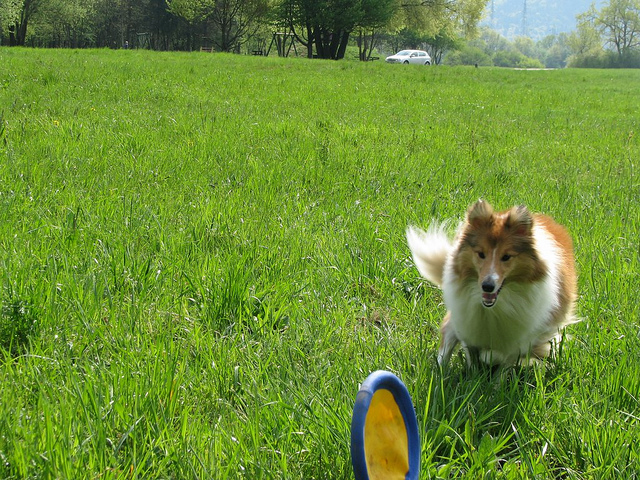
\includegraphics[width=2.5in]{imgs/example2_original.jpg}}
    \hspace{1mm}
    \subfloat[][Fixation map]{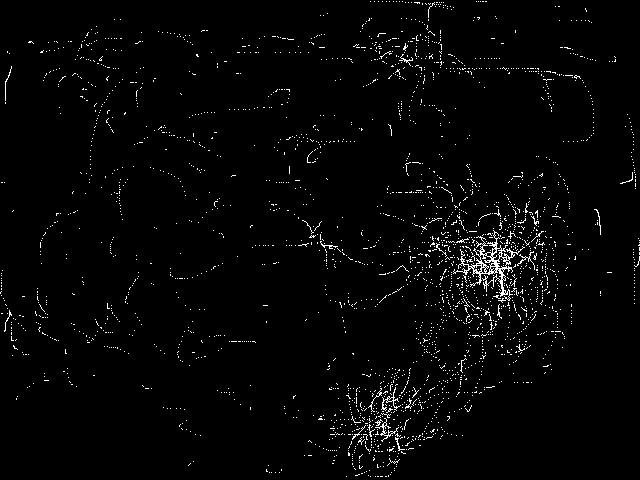
\includegraphics[width=2.5in]{imgs/example2_fixation.png}}
    \hspace{1mm}
    \subfloat[][Saliency map]{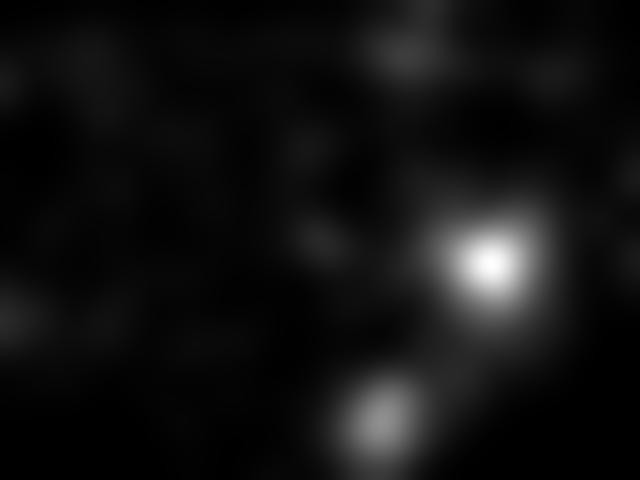
\includegraphics[width=2.5in]{imgs/example2_saliency.jpg}}
    \caption{Data example}
    \label{img:data_example_2}
\end{figure}

The CAT2000 contains 4000 images from 20 different categories. In those images, 2000 are for training and the other 2000
are for testing. There are 24 test subjects for each image and a total of 120 test subjects. The free 
viewing duration is 5 seconds. Fixation data from only 18 out of 24 test subjects are available in training
set, and the test set is released with only the original images.

The SALICON dataset is created using images from Microsoft Common Objects in Context (MS COCO) dataset\cite{linMicrosoftCOCOCommon2015}.
Instead of using an eye-tracker, mouse trajectories from different viewers are used in this dataset 
to calculate probability distribution of visual attention. A total of 20000 images from 80 categories, including
10000 in training set, 5000 in validation set, and 5000 in test set.
In training set, the original images, fixation maps, and saliency maps are all available, while 
the test set is released without fixation maps and saliency maps.


We plan to combine the training and validation set of SALICON, 
and split it into 10 folds (7 for training, 2 for validation, and 1 for testing). 
Our training data are the 7 folds from SALICON.
Our validation data for tuning the hyper-parameters is the other 2 folds from SALICON, 
and our testing data consists the remaining 1 fold from SALICON together with CAT2000.

Some datasets might not have groundtruth saliency maps available, and different dataset might use different gaussian standard variance to create the saliency maps.
So we need to generate saliency maps using a set of uniformed parameters from fixation data.

All images are resized to $256 \times 256$ and normalized using mean ($[0.485, 0.456, 0.406]$)and standard deviation ($[0.229, 0.224, 0.225]$).


\subsection{Interpretability}

The visual saliency algorithm takes an input of the original figure, and outputs a saliency map of the same size. Each pixel contains a float number from 0 to 1. Bigger numbers show that these pixels or areas get more focus. Therefore, it is a regression task and the output can be visualized by plotting the saliency map. From the visualization, we can intuitively judge whether the output saliency map corresponds with real data from people to check its interpretability.

However, there are several questions about interpretability that we need to answer if our implementation of attention mechanism works. The methods to check the results we suppose are detailed described in the "Further Verification" section.

\begin{itemize}
    \item The deep neural network is very powerful and can fit complex functions. If we insert a layer for attention, how should we confirm that adding these layers can effectively improve the performance, and their function cannot be replaced by other simpler layers (like fully connection layers) or being integrated into other layers?
    \item If the performance is good, how should we learn whether the final result depends largely on the attention layer, since its function is to assign some weights to some features?
    \item We previously assume that the attention layers help the network to focus on global information and cooperates with convolutional layers that focus on local features. How can we find evidence for this assumption?
\end{itemize}

\section{Analysis}
\subsection{Algorithm}
We choose CNN to predict the saliency maps. The filters in CNNs function as feature extractors,
and as the depth of the convolutional layer go up, the features tend to be more sophisticated
and high level. If we have learnable parameters assigned to different filters, the model can
learn to predict which features are more attractive to humans. 
This feature of CNNs fits our need of detecting visual saliency and it is the reason that we 
chose CNN.

We use UNet \cite{ronnebergerUNetConvolutionalNetworks2015} as the backbone of our model. UNet has a symmetric expanding path, made of
several skip connections, that enables precise localization. This feature can help assign correct visual saliency values 
to the corresponding locations. It also enables UNet to incorporate both low level features and
high level features. The structure of our model is shown in \ref{img:network}. The numbers under each
module indicate the width of the convolutional layer (number of filters/kernels) and determine the length of each module on the x-axis. 
The area of the east/west face indicates 
the relative size of the resulting image/feature map of that module. 
\begin{figure}[!h]
    \centering
    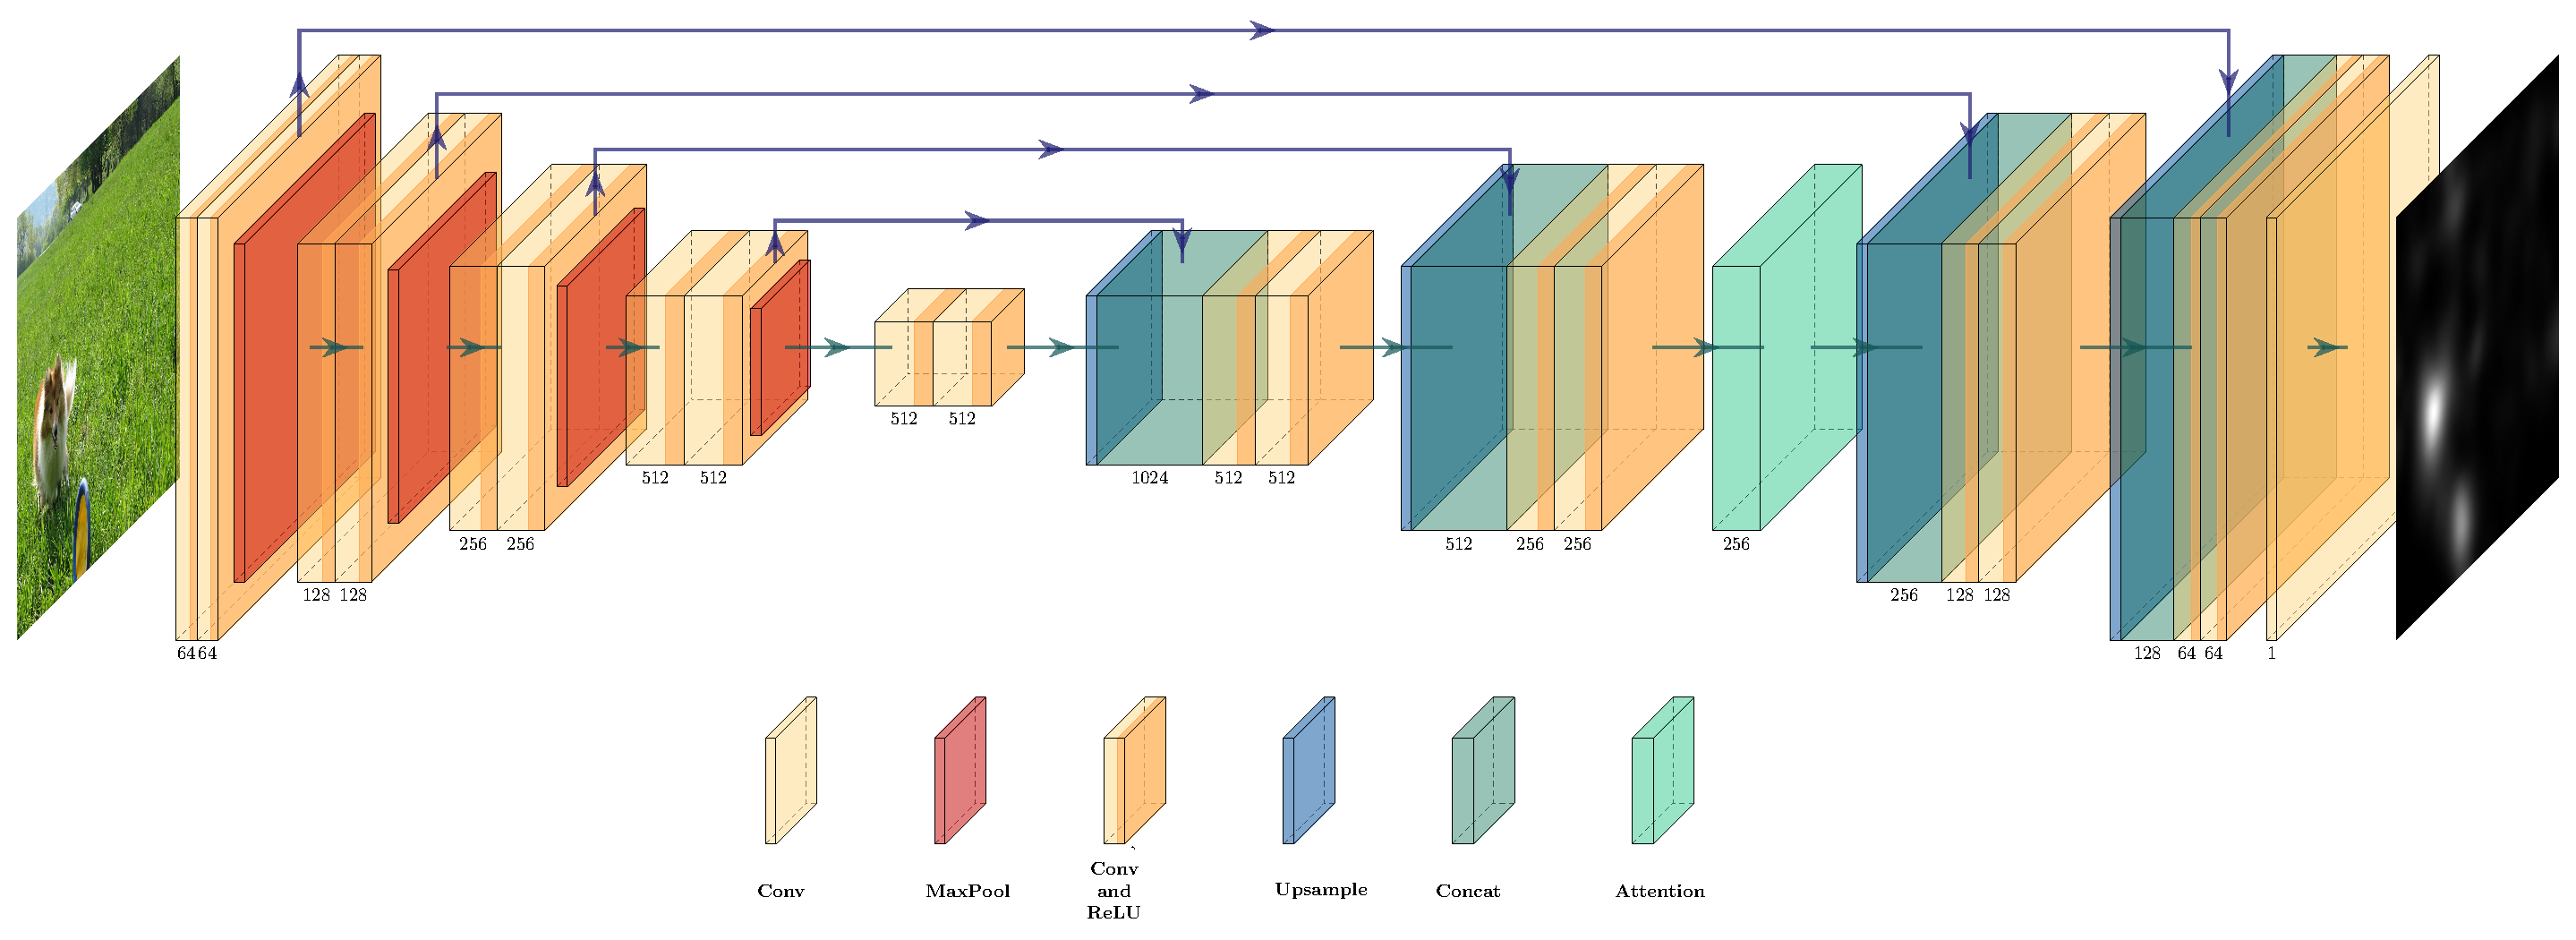
\includegraphics[width=7in]{imgs/network.pdf}
    \caption{Network structure}
    \label{img:network}
\end{figure}

As for the attention mechanism, we implement it as a Pytorch module, and then make this module
part of UNet's data path. The goal of this module is to find long distance dependencies across 
different parts in the image. The reason for introducing this module is that CNNs have a limited
reception field decided by the sizes of convolutional kernels, and we hope to alleviate this problem
by using attention mechanisms. We use the similar attention module described in 
\cite{zhangSelfAttentionGenerativeAdversarial2019a}, and the sturcture of the attention module is shown in
\ref{img:attention}. The attention map is a $1 \times N \times N$ tensor, where $N$ is the total number of 
pixels in the output of $f(x)$ (or $g(x)$, they output tensors of the same size). This map acts like a 
relationship matrix, where each element in the matrix indicates the bond/dependency between two particular
pixels in the input feature map. However, applying this attention module directly on the original input
image will result in a huge attention map which would consume a lot of memory and make the calculations
expensive. Therefore we put this module in the middle part of the network, where the feature map is relativly
small. We also reduced the number of kernels of $f(x)$, $g(x)$, and $h(x)$ to further reduce the memory 
usage and speed up the execution.

\begin{figure}[!h]
    \centering
    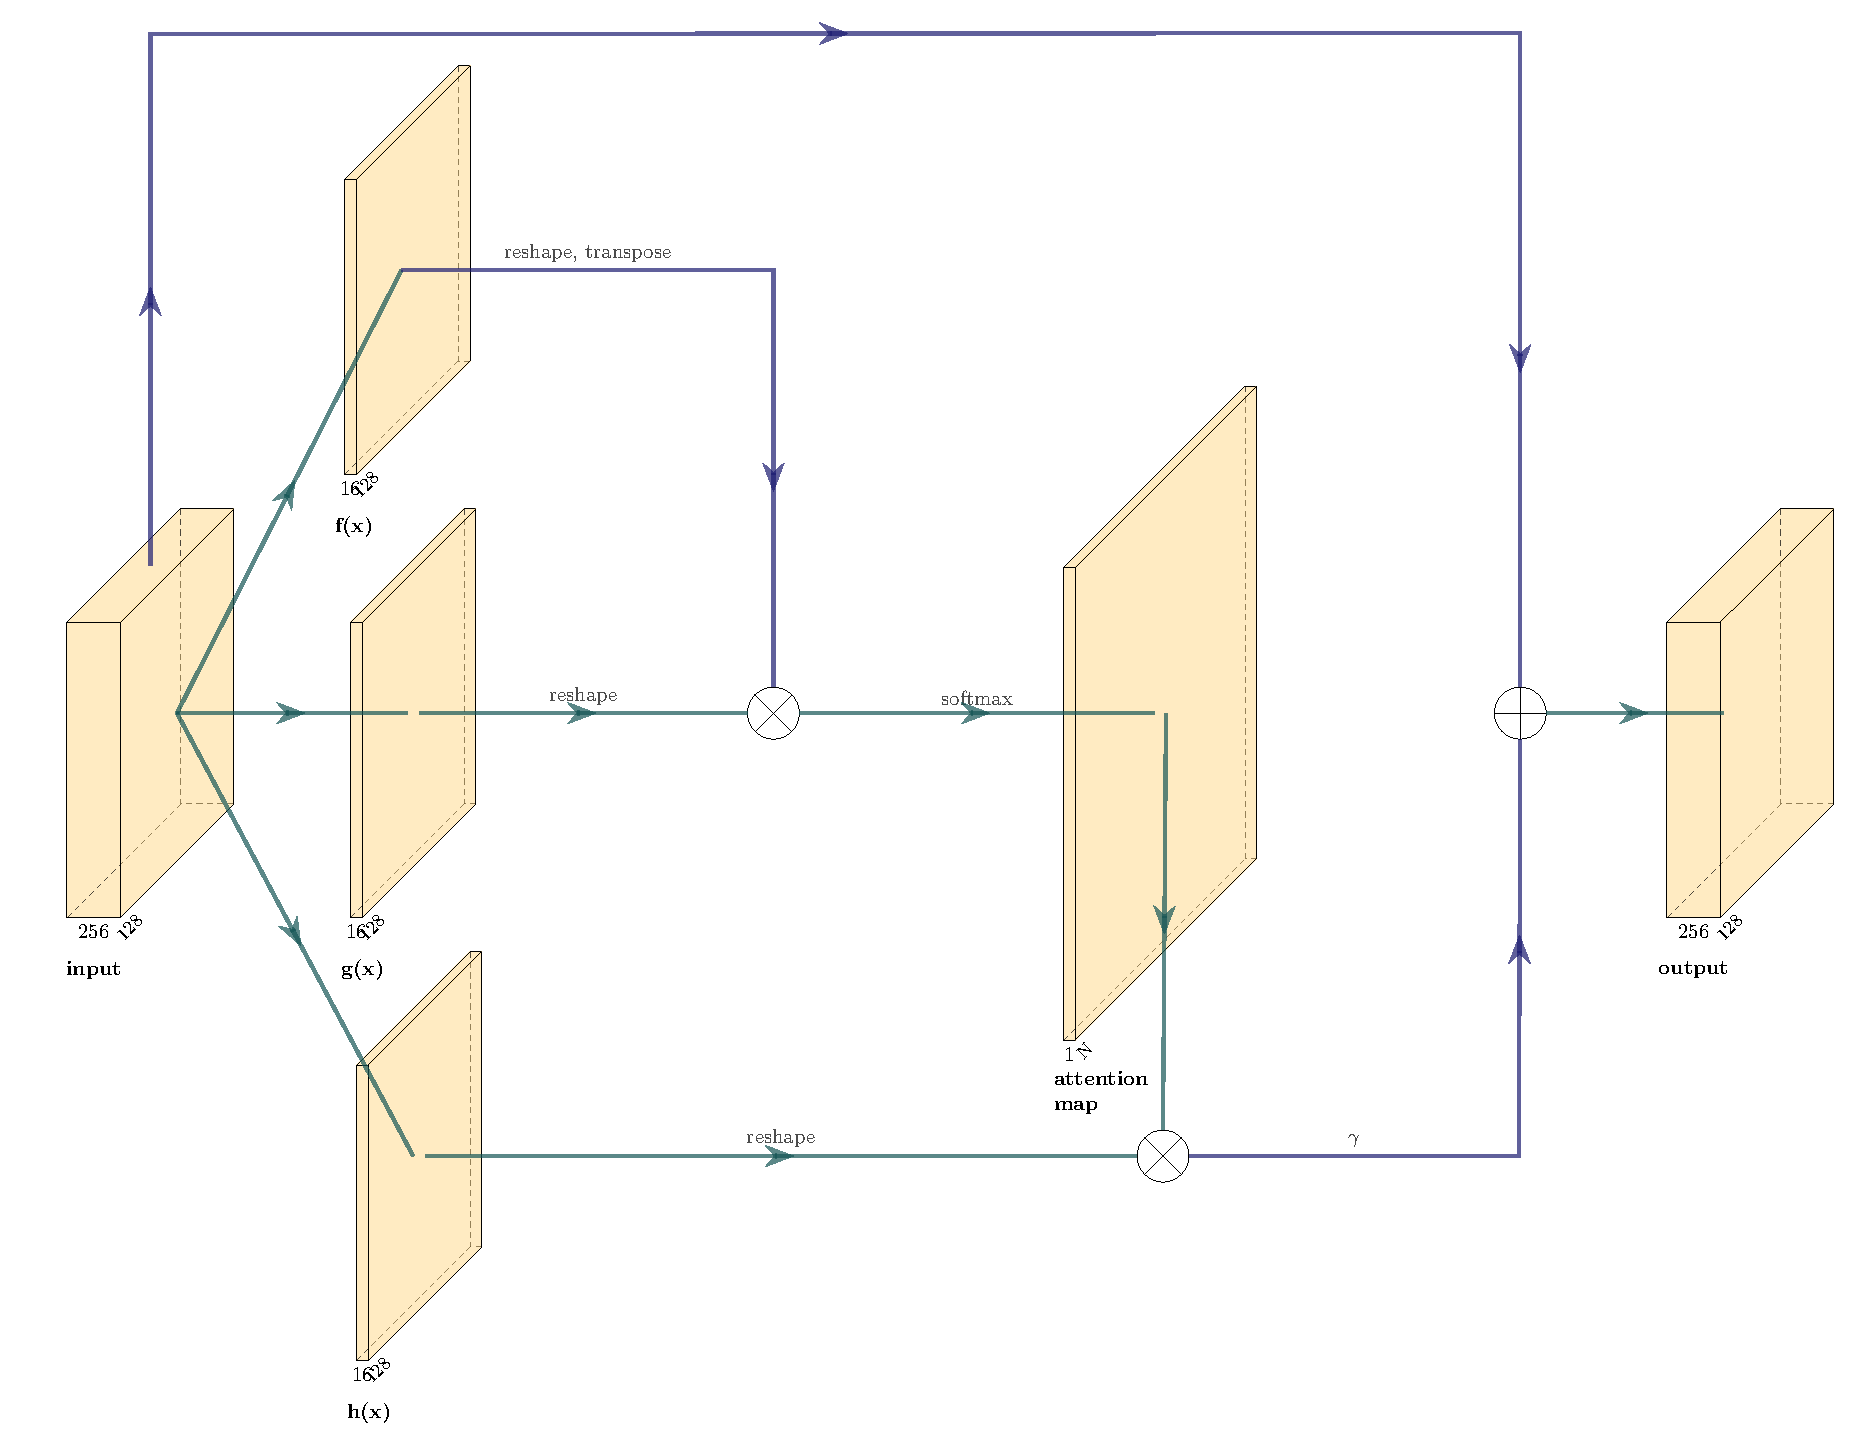
\includegraphics[width=4in]{imgs/attention.pdf}
    \caption{Attention module structure}
    \label{img:attention}
\end{figure}


Since this is an end-to-end model, the dataflow will be pretty straightforward. The input data is fed to the model,
and then the output is compared with groundtruth to compute the loss. The loss is then back propagated to update model parameters.

Since the ground truth of the test set of these datasets are not public, we will divide the original dataset into the train set, the validation set and the test set. We can choose suitable hyper-parameters based on the results of the train set and the validation set.

\subsection{Performance Measurement}

There are several metrics that can be used to measure the performance. According to \cite{riche2013saliency}, these various metrics may reflect different properties of the algorithm.
\begin{itemize}
    \item Normalized scanpath saliency (NSS \cite{petersComponentsBottomupGaze2005})
    \item Correlation coefficient (CC)
    \item Area under receiver operating characteristic curve(AUC \cite{richeSaliencyHumanFixations2013})
    \item etc.
\end{itemize}

The NSS measures the mean saliency value at fixated locations of the normalized (zero mean, unit variance) saliency map. 
It can be calculated using Eq. \ref{EQ:NSS}. 
\begin{equation}
    \begin{aligned}
        NSS &= \frac{\sum^{N} T_{i}}{N}\\
        \text{where }T &= \frac{S - \bar{S}}{\sigma_{S}} \circ F
    \end{aligned}
    \label{EQ:NSS}
\end{equation}
In this equation, $S$ is the saliency map, $\bar{S}$ is the mean of $S$, $\sigma_{S}$ is 
the standard deviation of $S$, $F$ is the fixation map with only $0$ and $1$ as pixel values in it,
$T_{i}$ is the pixel value in $T$ at location $i$, and $N$ is the total number of non-zero pixels in $F$.

The CC is the linear correlation coefficient between a model saliency map and an empirical saliency map 
gained from convolving the fixation locations with a Gaussian kernel. It can be calculated using EQ. \ref{EQ:CC}. 
\begin{equation}
    \begin{aligned}
        CC = \frac{\sum_{i=1}^{n}(x_{i}-\bar{x})(y_{i}-\bar{y})}
        {\sqrt{\sum_{i=1}^{n}(x_{i}-\bar{x})^{2}}\sqrt{\sum_{i=1}^{n}(y_{i}-\bar{y})^{2}}}
    \end{aligned}
    \label{EQ:CC}
\end{equation}


In AUC metric,
the saliency map is treated as a binary classifier to separate positive from negative samples at various thresholds. 
The true positive (TP) rate is the proportion of saliency map values above threshold at fixation locations. 
The false positive (FP) rate is the proportion of saliency map values above threshold at all pixels. 
We calculate the TP rate and FP rate using a series of thresholds between $[0, 1]$, and draw a
receiver operating characteristic (ROC) curve with FP rate as x-axis and TP rate as y-axis.
An example of this curve is shown in Fig. \ref{img:AUC} \cite{hanleyMeaningUseArea1982}.
The area under this curve is reported as AUC.
\begin{figure}[!h]
    \centering
    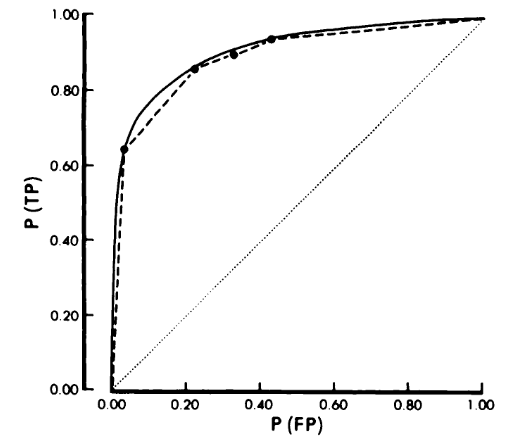
\includegraphics[width=2.5in]{imgs/AUC.png}
    \caption{ROC curve example\cite{hanleyMeaningUseArea1982}}
    \label{img:AUC}
\end{figure}


The performance is reported on the testing fold of SALICON and also the whole CAT2000 dataset.
Reporting scores using different datasets can make the results more convincing,
because it can show that our model can generalize well.

\subsection{Hyperparameters}
The hyper-parameters that need to be tuned are:
\begin{itemize}
    \item loss function to use,
    \item learning rate.
\end{itemize}

The loss functions we experimented with are:
\begin{itemize}
    \item mean square error (MSE),
    \item NSS,
    \item CC.
\end{itemize}
For learning rate we experimented with $0.01$ and $0.001$.

\section{Results}
We use Pytorch Lightning framework \cite{falcon2019pytorch} to implement our project. Our code (including \LaTeX files for this
report) is available at \href{https://github.com/Freddiechang/CMPUT566}{our GitHub repo page}.
The model is trained for 200 epochs under each hyperparameter setting. The performance scores are listed in Table \ref{tbl:performance}.
\begin{adjustwidth}{0cm}{0cm}
\begin{table}[!h]
    \begin{tabular}{cc|cccc}
        \hline
        Loss function & Attention module & NSS(SALICON) & CC(SALICON) & NSS(CAT2000) & CC(CAT2000)\\
        MSE(3) & Yes & 1.1585 & 0.8514 & 1.5873 & 0.6063\\
        MSE(2) & No & 1.1639 & 0.8564 & 1.5980 & 0.6102\\
        CC(2) & Yes & 1.1624 & 0.8556 & 1.5979 & 0.6120\\
        CC(1) & No & 1.1725 & 0.8624 & 1.6169 & 0.6185\\
        NSS(1) & Yes & 0.8871 & 0.5984 & 1.2306 & 0.4399\\
        \hline
        \multicolumn{2}{c}{SALICON average} & 1.5691 & 1 & NA & NA \\
        \multicolumn{2}{c}{CAT2000 average} & NA & NA & 2.97 & 1 \\
        \hline
    \end{tabular}
    \caption{Performance under different settings. The numbers in the brackets after the loss function names indicate
    how many experiments we did under this setting, and the average performance is reported. We also calculated the performance
    baseline using the groundtruth fixation maps and saliency mapd from the datasets, and the scores are reported in SALICON average
    and CAT2000 average rows.}
    \label{tbl:performance}
\end{table}
\end{adjustwidth}


















% not sure if we should keep this part
\subsection{Further Verification}

The first verification is the pre-training modification. We use the same series of training samples to train two models. One of them is with the attention layer. The other replaces this layer with a simple one (e.g. fully connection layer). Then we will compare the training process, including the convergence speed, the loss change and the final performance measured by different metrics. If the attention mechanism is simple enough and can be easily replaced by other layers or integrated into the network, then it does not have any specialties.

The second verification is the post-training verification. Namely, during test, we will disable the attention layer or add random noise and compare the final performance with the output of the normal framework. This step will check the contribution and importance of the attention layer. If the metrics to measure the performance have different levels of changes, we can infer about the properties of the attention layers according to the characteristic of these metrics.

We are also interested in what information in the picture is used by the algorithm to calculate the output. Some pixels, like local sharp margins of the objects, may help locate the focused area, but may not be themselves focused. A large area of the same color in the middle may be coded as global information and help the network to distract attention to more important parts of the pictures.
We might use the Integrated Gradients algorithm (IG) \cite{sundararajan2017axiomatic} to analyze what pixels in the picture contributes to the result. The algorithm does the following thing: Make the figure slowly change from a totally black or grey background to the original figure.
After each step of changing, we calculate the gradients of a critical value to all the pixels. (This critical value can be the sum of the values of the highly focused pixels.) We can integrate these gradients (sum and multiply by pixel changes) to show which pixels have the most contribution to the final result during changing.
It might be interesting if we can find some pixels that are not highlighted in the saliency map but help the machine to focus. 
During this process, we can also monitor our network's sensitivity to dimmed picture and explore whether it corresponds with human feelings. 

If time permitting, we are going to test whether the position of the attention layer will change the result. We can explore whether the attention layer works well on simple or complex features based on the depth of the network.



\section{Task Distribution}
Credits for implementation:
\begin{itemize}
    \item training, validation and test procedure (Shupei)
    \item SALICON data handling (Shupei)
    \item CAT2000 data handling (Sijie)
    \item FIGRIM and Fillers data handling (Mehdi)
    \item loss functions: NSS, CC, shuffled AUC, AUC-Borji, and AUC-Judd (NSS and CC implemented by Shupei, all AUC methods implemented by Mehdi)
    \item attention mechanism module (Shupei)
    \item integrated gradients algorithm framework (Sijie).
\end{itemize}

Credits for experiment:
\begin{itemize}
    \item training (Shupei and Mehdi)
    \item testing (Shupei and Sijie)
    \item analysis (Sijie)
\end{itemize}

% needs update
Credits for this report:
\begin{itemize}
    \item introduction (Shupei)
    \item related work (Shupei)
    \item datasets (Shupei and Sijie)
    \item interpretability (Sijie and Shupei)
    \item algorithm (Shupei and Sijie)
    \item performance measurement (Shupei and Sijie)
\end{itemize}
Mehdi proofread and revised the whole document.




\subsection{Future Plan}
Step1: Before the March 11 checkpoint, we are going to write the code of the CNN network and applies attention mechanism to it. Coding work has already been finished by Shupei and Mehdi and the code is running smoothly.

Step2: For the first week after the checkpoint, we are going to use the validation set to choose good parameters of the network to achieve better results. We also consider accelerating the matrix calculation of the attention layer in order to get the results faster in later steps.

Step3: For the second and third week after the checkpoint, we will mainly focus on interpretation tasks. This includes pre-training modification, post-training verification, and the integrated gradients method.

Step4: Before submission, if we finish the above steps early, we can try other things mentioned, including implementing another attention mechanism or change the position of the attraction layer in the network in order to find more properties of the attention layer.

%ethics
%biased dataset
%misuse: put some stuff in less salient region
%
\newpage

\bibliographystyle{unsrt}
\bibliography{proposal}


\end{document}
